We validated our methodology by developing a use-case concerning risk assessment for financial companies.
Our application is inspired on the ORCA System\footnote{The ORCA System is a trademark of GCP Global (www.gcpglobal.com).}.
Risk assessment is implemented by an interactive business process based on the exchange of a series of questionnaires intended to evaluate the risks implied the client's business practice.
For instance, the conditions and protocols used to perform confidential transactions, the physical security for accessing reserved areas such as computing server installations.
The information gathered by the questionnaires is used to determine whether there are risky practices within the business processes of the company, as well as to propose amends to these practices.
The ultimate goal of the risk assessment is to determine a degree of compliance to existing standards.
By analysing the questionnaires, ORCA detects risky practices, proposes solutions and triggers further assessment processes to ensure that the solutions have been implemented.

Our goal is to model a service based application (called \FlyingPig), for providing risk assessment as a service.
In order to provide this functionality, \FlyingPig\ would benefit from ORCA's legacy services: storage, assessment and data visualization functions.

In the following, we describe the results of applying $\Pi$-SODM to develop the \FlyingPig\ risk assessment system.
The models presented next were generated as a result of interacting with software developers at GCP Global.

\begin{figure}
\centering
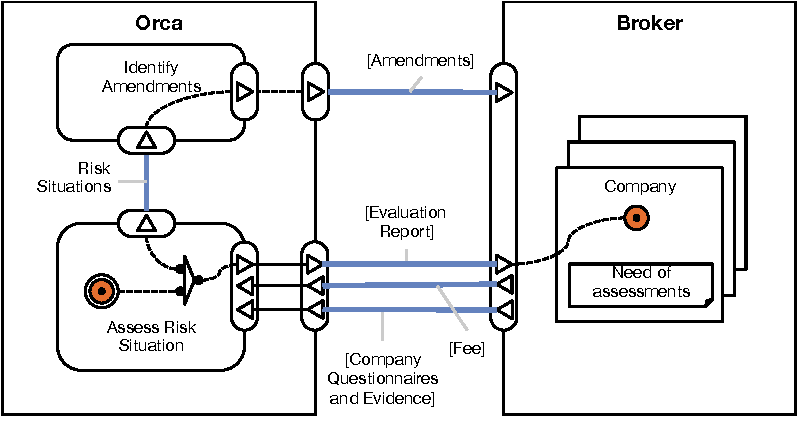
\includegraphics[width=0.7\textwidth]{figs/3ValueModel.pdf}
\hspace*{5cm}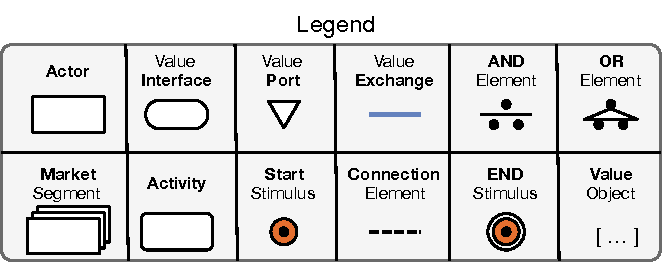
\includegraphics[width=0.4\textwidth]{figs/3ValueKey.pdf}
\caption{E3value model for \FlyingPig.\label{fig:E3valuemodel}}
\end{figure}


\subsection{Computation-Independent Models (CIM)}

$\Pi$-SODM uses two models at the CIM level: The E3value~\cite{e3value} model and BPMN~\cite{BPMN}.
The former  identifies the transference of value information between components of the system.
The BPMN model establishes which are the actors and main tasks of the application.

Figure~\ref{fig:E3valuemodel} shows the value model for the \FlyingPig\ application.
It is a business model that graphically represents a business case as a set of value exchanges ($\triangleright$ and $\triangleleft$) and value activities (rounded boxes) performed by business actors (squared boxes).

In our use-case, we identify two business actors: \textsl{ORCA} and \textsl{Broker}. 
Brokers are responsible for channelling requests for risk assessment of one or several companies. 
ORCA have two value activities which are services that provide an economical benefit: to \textsl{Identify Amendments} and the possibility to \textsl{Assess Risk Situation}. 
The values exchanged between ORCA and the brokers are: \textsl{Amendments} and \textsl{Evaluation Reports} which are value objects ([ \!\dots]) for the companies that need to have a risk assessment, as well as  \textsl{Questionnaire and Evidences} and the risk assessment \textsl{Fee} which are value objects for ORCA System.

The e3value defines \textit{dependency paths}, showing the value exchanges, which are triggered by the occurrence of an end-consumer need (in our case, the need of a risk assessment). 
A dependency path has a direction and consists of a sequence of linked dependency nodes.
A dependency path starts with a \textit{start stimulus} node and ends with an \textit{end stimulus} node (see Legend on Figure~\ref{fig:E3valuemodel}). 
Dependency paths may also contain \textsl{OR} and \textsl{AND} elements (both for initiate and join alternative and parallel paths).

The dependency path in Figure~\ref{fig:E3valuemodel} initiates with the need of assessment by a particular company. 
Once this need occurs, the value exchanges between ORCA and Broker are triggered. 
The client company will provide orca wit information (answers to a questionary), evidence (to support the information) and a fee (monetary value).
ORCA will provide amendments (recommendations to change practices) and an evaluation report. 

\begin{figure}[t]
\centering
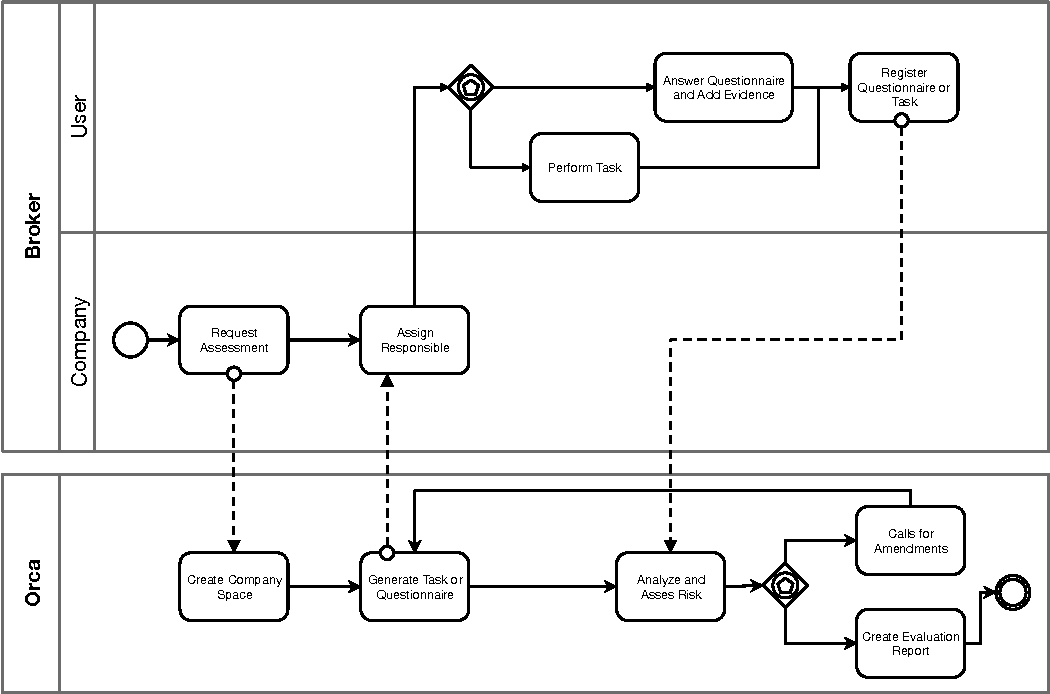
\includegraphics[width=1.0\textwidth]{figs/BPMN_GCP.pdf}

{\color{red} Javier: Please change \underline{Asses} by \underline{Assess}. --M}
\caption{BPMN model for \FlyingPig.\label{fig:BPMNmodel}}
\end{figure}

The BPMN model is devised to better understand the process in which the value exchanges occur.
Figure~\ref{fig:BPMNmodel} shows the BPMN model\footnote{Details on BPMN (Business Process Management Notation) can be found in http://www.bpmn.org/.} for the \FlyingPig\ scenario. 
The model includes two pools representing the \textsl{ORCA} system and the \textsl{Brokers}. 
Brokers have two lanes, the client \textsl{Company} and a \textsl{User}. 
The user is a contact member of the company, who will coordinate the assessment process. 
This process will involve other members of the company as well.

The risk assessment process starts after a request from a company.
(This agrees with the value model, in which the start stimulus triggers the whole process.)
The request leads to the definition of a group of users that will answer questionnaires for evaluating risk.
Questionnaires are considered tasks that users will have to perform. 
Other tasks include amending a ``risky situation'' as well as producing evidence to show that a specific risk has been eliminated\footnote{Risky situations include from physical facts such as not having easy access to handicapped persons or having an unsecured access to the premises of the company, to more intangible ones, such as the use of an less-than-optimal protocol to access data on the company's computer server.}.

Once tasks are completed, they are stored and analysed to generate a list of un-compliant situations, associated to their corresponding \textit{calls for amendment}, in case there are any, or a report specifying a compliance level, incidents and a risk map.
During the process of analysing a questionnaire, the answers of some questions can trigger the generation of other questionnaires or amendments, that will become new tasks.  

Business processes have also associated rules and constraints that define their non functional requirements.
NFR represents the ``semantics'' and the conditions in which the tasks must be done.
In our example we have some constraints.

{\color{red}
Placido, Valeria: What can we say about non-functional requirements at the CIM level?
}

\subsection{Platform-Independent Models (PIM)}

In Section~\ref{sec:modelingWithPISODM} we defined three models at the PIM level.
These models are built next, for the \FlyingPig\ scenario.

\begin{figure}[t]
\centering
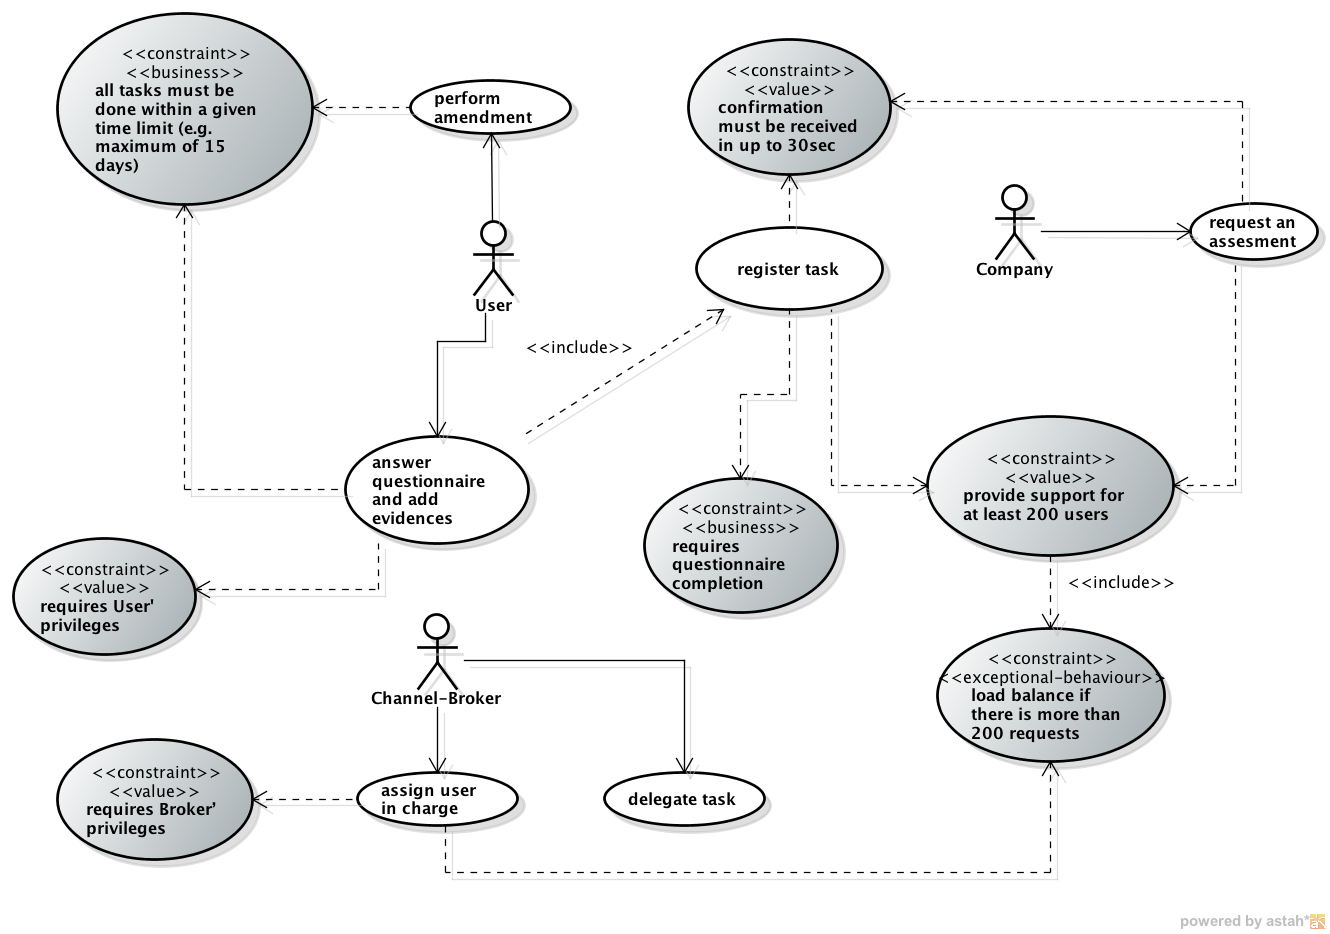
\includegraphics[width=0.9\textwidth]{figs/UseCaseGeneral.png}

{\color{red} \raggedright
$\star$ ``Create a responsible'' should be changed for ``Designate user in charge''.

$\star$ ``requires concurrency for more than 200 users'' should be changed by ``Maximum number of users should be greater than 200''.
}
\caption{$\pi$-UseCase model for \FlyingPig.\label{fig:piUseCaseModel}}
\end{figure}


\paragraph{\underline{$\pi$-UseCase Model for \FlyingPig}}~

The $\pi$-UseCase model shown in Figure~\ref{fig:piUseCaseModel} describes the features and constraints for the \FlyingPig\ application. 
In this model, three actors are identified: \textit{Company}, \textit{User} and \textit{Channel-Broker}\footnote{\color{red} Can we change this for Broker ? --M.}. 
They are represented as stick figures.
In the context of \FlyingPig, Company is the actor asking for risk evaluation.
A Channel-Broker is the responsible for channelling the the evaluation process, assigning users to be in charge of tasks as well as delegating tasks. 
A User, in this model is an actor who answers questionnaires (with base on the actual facts about the Company).
The User also produces evidence to support facts and performs the necessary amendments to improve the results of the risk assessment.

Each actor is associated to one or more use cases (depicted as white ovals in Figure~\ref{fig:piUseCaseModel}). 
Use cases describe the main functionalities of the system.
The $\pi$-UseCase model for \FlyingPig\ defines six use cases. 

In our model, each use case may be associated to one or more (non-functional) constraints (depicted as coloured ovals in Figure~\ref{fig:piUseCaseModel}). 
The model defines three types of constraints: \textit{value} , \textit{business} or \textit{exceptional behavior}. 
Each constraint is identified by the word $<<$\textsf{constraint}$>>$ followed by its type.

In the case of \FlyingPig, the model counts seven constraints:
\begin{numtrivlist}
\item An acknowledgement is due less than 30 seconds after registering a task or demand for assessment. 
\item The system's infrastructure should be prepared to deal with, at least, 200 users. 
\item If the number of requests exceeds 200, \FlyingPig\ should make a load balance of the requests. 
\item The Channel-Broker must have their privileges verified \textit{before} the execution of the actions associated to the \textsf{designate user in charge} use case.
\item Users must have their privileges verified \textit{before} the execution of the actions associated to the \textsf{answer questionnaire and add evidences} use case.
\item All questionnaires need to be fully answered, in order to consider that a task is completed.
\item There is a time limit (in days) for each amendment required by the system.
\end{numtrivlist}

{\color{red} Anything else here? --M}

\begin{figure}
\centering
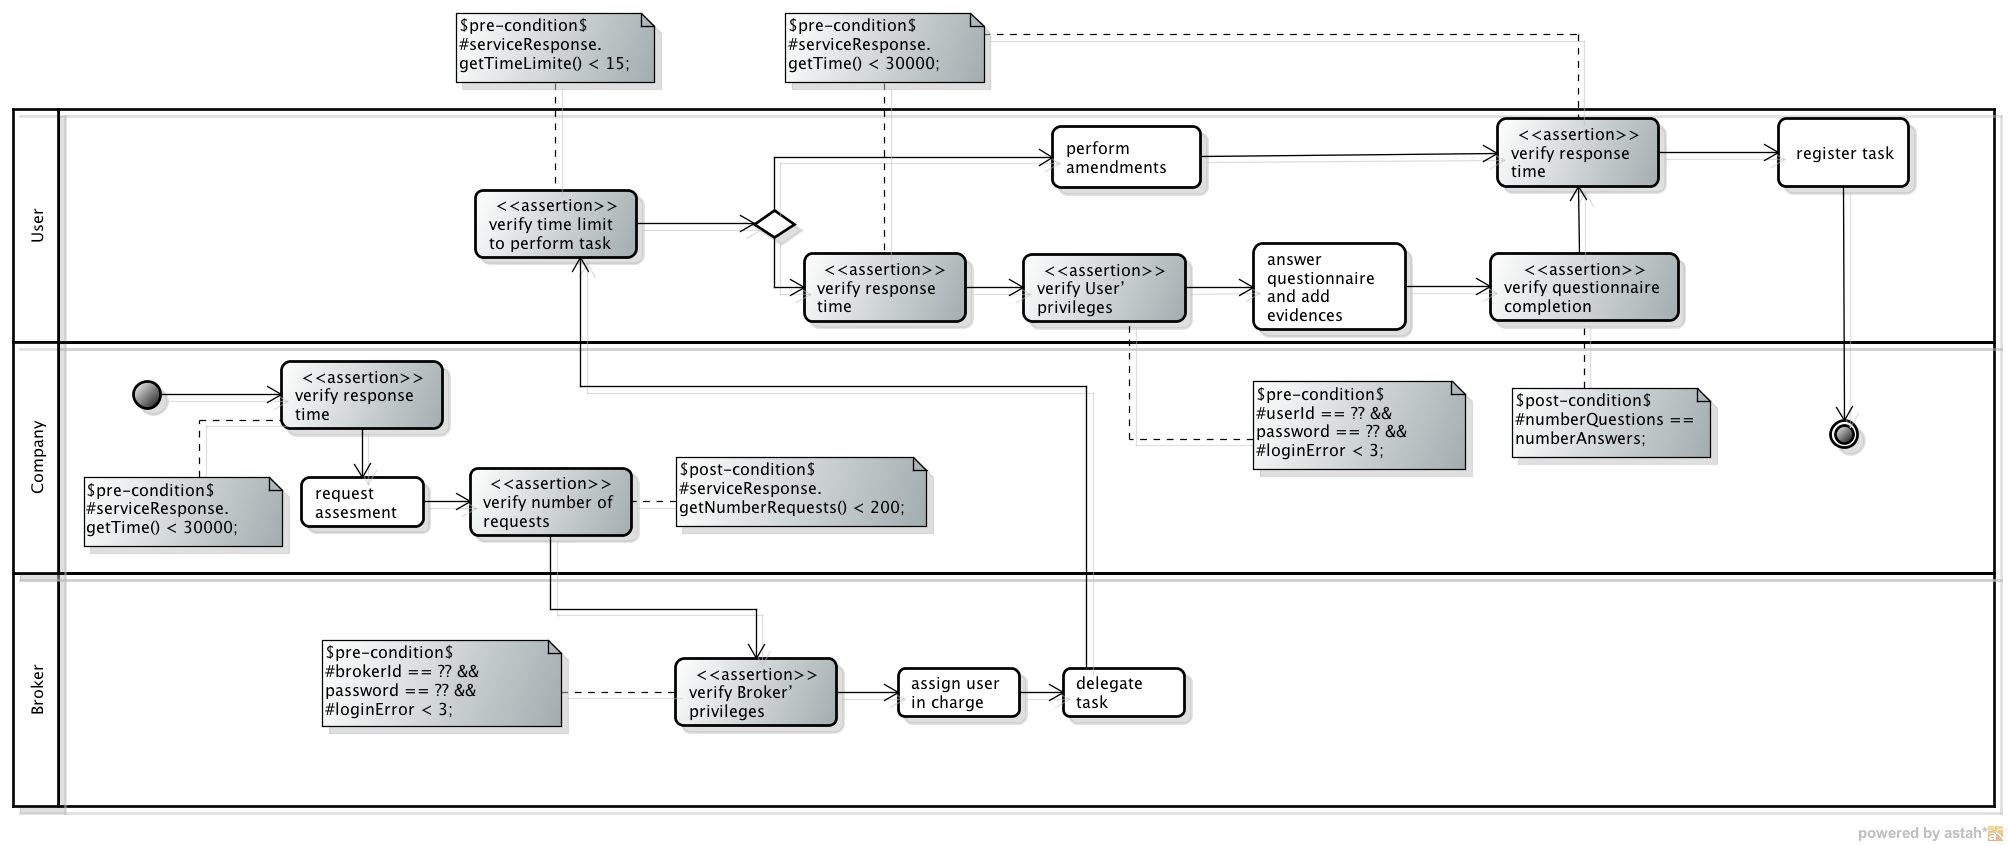
\includegraphics[width=1.0\textwidth]{figs/ServiceProcessGeneralCut.png}
\caption{$\pi$-ServiceProcess model for \FlyingPig.\label{fig:PiServiceProcessModel}}
\end{figure}

\paragraph{\underline{$\pi$-ServiceProcess Model for \FlyingPig}}~

The $\pi$-ServiceProcess model (Figure~\ref{fig:PiServiceProcessModel}) presents the workflow for \FlyingPig.
The actions in this model were obtained by applying the use case transformation rules described in Section~\ref{sec:pewsmetamodel}.

The \textsf{Company}, \textsf{Broker-Channel} and \textsf{User} actors are transformed into lanes that represent the business collaborators.
Use cases are transformed into \textit{actions} and are represented by white boxes.
The restrictions associated to each use case are transformed into \textit{assertions} (represented by coloured boxes) and may be decorated with pre- and post-conditions. 
We can see that this model refines the concepts defined in the $\pi$-UseCase model.
The assertions specify those non-functional requirements, as they are seen by the actors. 
The next step in the development is to add these assertions to the models that specify the \FlyingPig\ system.

\begin{figure}[t]
\centering
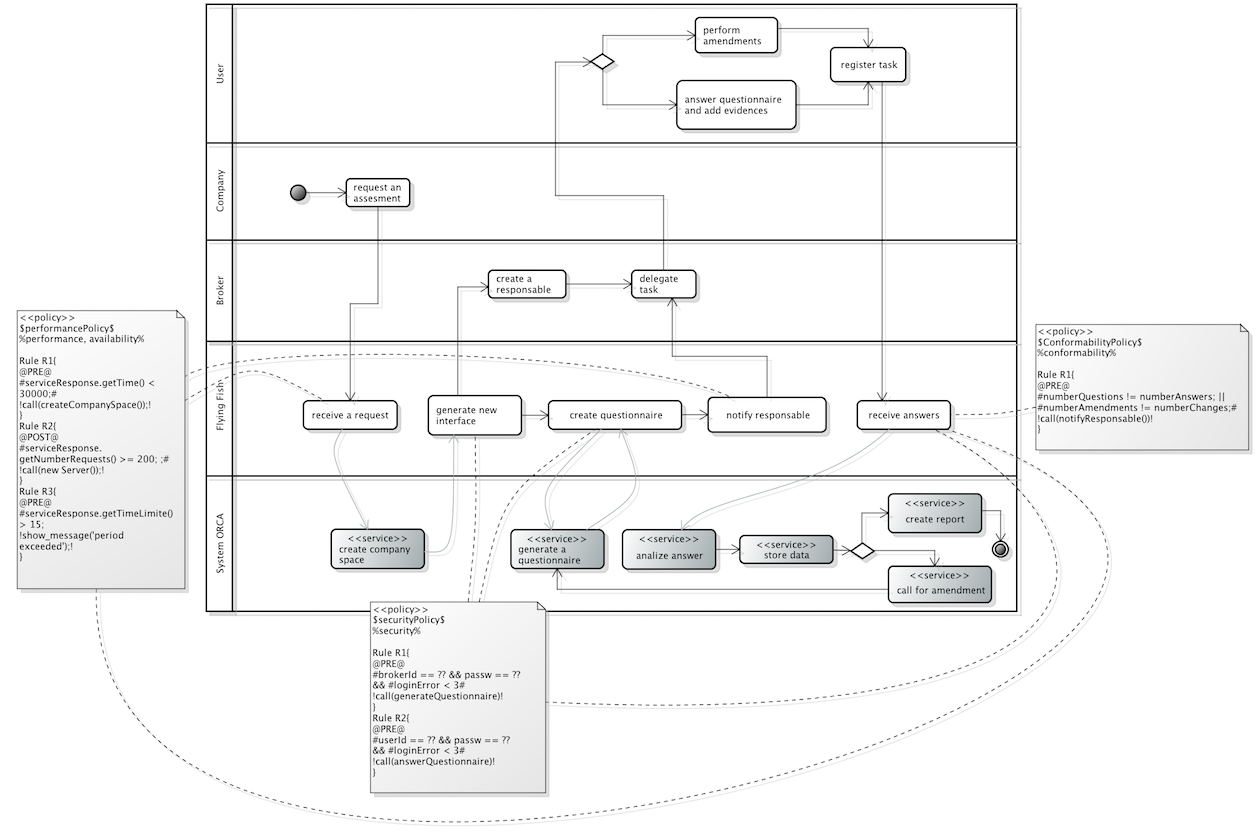
\includegraphics[width=1.0\textwidth]{figs/ServiceCompositionGeneralCut.png}
{\color{red} \raggedright
$\star$ Change FlyingFish by \FlyingPig.
}
\caption{$\pi$-ServiceComposition model for \FlyingPig.\label{fig:PiServiceCompositionModel}}
\end{figure}

\paragraph{\underline{$\pi$-ServiceProcess Model for \FlyingPig}}~

The model presented in Figure~\ref{fig:PiServiceCompositionModel} offers a system-centric view of the application.
The previous model is now enhanced with a view of the \FlyingPig\ application, including those services upon  it is build.
The assertions in Figure~\ref{fig:PiServiceProcessModel} are implemented as \textit{policies}.
These policies contain the pre- and post-conditions of the previous model.
They are associated to actions of the system.


\begin{figure}[t]
\centering
%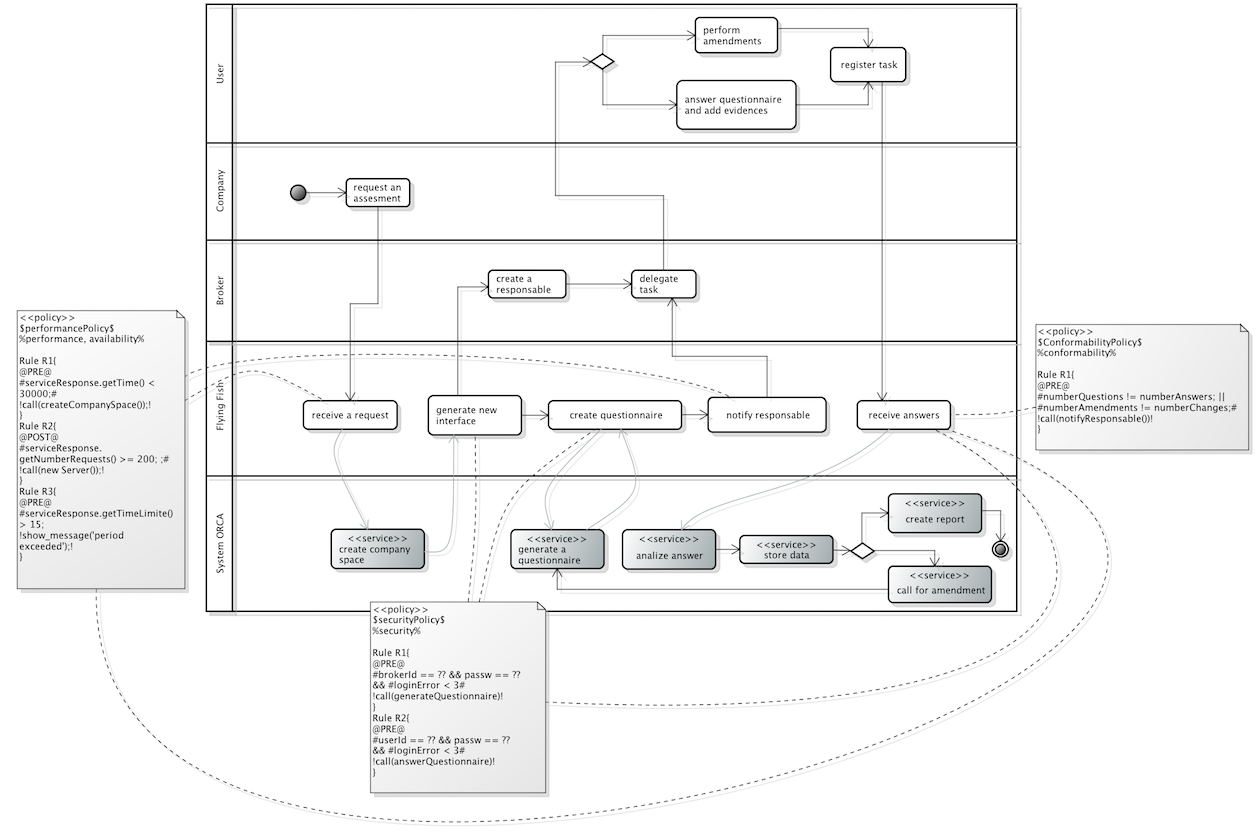
\includegraphics[width=1.0\textwidth]{figs/ServiceCompositionGeneralCut.png}
\fbox{\LARGE $\pi$-PEWS Model.}

{\color{red} \raggedright
$\star$ Placido: Please, place the model here.
}
\caption{$\pi$-PEWS model for \FlyingPig.\label{fig:PiPEWSModel}}
\end{figure}

\subsection{Platform-Specific Model (PSM)}

The model presented in Figure~\ref{fig:PiPEWSModel} is the result of translating the previous model into service composition code.
Notice that the workflow for \FlyingPig\ is implemented by using the constructors present in BPEL~\cite{BPEL}, with the addition of the notion of \textit{contract}.

Contracts may be implemented as transversal concerns~\cite{aspects}.
Their conditions may be verified at specific point of the composition and their actions are executed if needed.

%%%%%%%%%%%%%%%%%%%%%%%%%%%%%%%%%%%%%%%%%%%%%%%%%%%%%
\subsection{Lessons Learned}

Through the example we underlined that every application implements functional aspects that describe its application logic.
Recall that an application logic refers to routines that perform the activities to reach the application objective.
Also there are non functional properties derived from NFR. They refer to strategies to be considered for the application execution like: security, isolation, adaptability, atomicity, and more.
These non functional properties must be ensured at execution time, and they are not completely defined within the application logic.

The challenge is to define them and to associate them with the application logic considering that different to existing solutions that suppose that it is possible to access the execution stat of all the components  of an application and that the application has complete control on them, in the case for service oriented applications  the components are autonomous services
API does not necessarily export information about methods dependency (e.g., in the REST protocol);
they do not share their state (stateless).

Given a set of services with their exported methods known in advance or provided by a  service directory, building services' based applications can be  a simple task that implies expressing an application logic as a services' composition. The challenge being  ensuring the compliance between the specification and the resulting application. Software engineering methods (e.g., \cite{1,2,decastro1,PapazoglouH06}) today can help to ensure this compliance, particularly when information systems include several sometimes complex business processes calling Web services or legacy applications exported as services.

As WS-* and similar approaches, our work enables the specification and programming of crosscutting aspects (i.e., atomicity, security, exception handling, persistence).
In contrast to these approaches, our work specifies policies for a services composition in an orthogonal way. Besides, these approaches suppose that non-functional properties are implemented according a the knowledge that a programmer has of a specific application requirements but they are not derived in a methodological way, leading to ad-hoc solutions that can be difficult to reuse. In our approach, once defined the policies for a given application they can be reused and/or specialized for another one with the same requirements or that uses services that impose the same constraints.